% HEADER and settings -- do not change
\documentclass[final,a4paper]{aust_thesis}
\usepackage{definitions}
\usepackage{graphicx}
\usepackage{float}
\usepackage{subcaption}
\usepackage[linesnumbered,ruled,vlined]{algorithm2e}
\usepackage{algpseudocode}


% The set of languages we want to show
\lstloadlanguages{Python}

% one can select one...
\lstset{language=Python}


%%%%%%%%%%%%%%%%%%%%%%%%%%%%%%%%%%%%%%%%%%%%%%%
%%!!          THIS WILL BE CHANGED       !!%%%%

%%   FRONT MATTER  
\submityear{%
2019%
}
\submitmonth{%
June%
}
\title{%
Fast and Accurate Feature-based Region Identification
}
\author{%
Maduakor Francis
}
\tutor{%
Prof. dr. Lehel Csat\'o\\
~\\
Faculty of Mathematics and Informatics,\hspace*{-3cm}\\
Babe\c{s} Bolyai University of Cluj-Napoca,\hspace*{-3cm}\\
Romania
}

% this is to speed up compilation...

%\includeonly{intro}


\begin{document}
% begin approval page
\begin{figure}[h]
	\centering
	\pgfimage[width=0.7\linewidth]{images/logo_approval}
\end{figure}



\begin{center}
	\large\textbf{Approval by}
\end{center}
\leavevmode\\
\leavevmode\\
\leavevmode\\
\leavevmode\\
\noindent
\textbf{Supervisor}\\
Surname:\\
First name:\\
Signature:\\
\\
\\
\\
\\
\noindent
\textbf{The head of department}\\
Surname:\\
First name:\\
Signature:\\


\vspace*{\fill}
\begingroup
\begin{center}
	\tiny KM 10, Airport Road, Galadimawa. Abuja – Nigeria. P.M.B 681, Garki-Abuja. Tel: +234 (0) 9 291 6265 -7
	www.aust.edu.ng
\end{center}
\endgroup
%%%% end approval page




\pagebreak
\vspace*{\fill}
\begingroup
\centering

COPYRIGHT \textcopyright 2019\\
MADUAKOR UGOCHUKWU FRANCIS\\
ALL RIGHTS RESERVED\\

\endgroup




%% ABSTRACT
\begin{abstract}%

\noindent There have been several improvement in object detection and semantic segmentation results in recent years. Baseline systems that drives these advances are Fast/Faster R-CNN, Fully Convolutional Network and recently \textbf{Mask R-CNN} and its variant that has a weight transfer function.  Mask R-CNN is the state-of-art.  This research extends the application of the state-of-art in object detection and semantic segmentation in drone based datasets. Existing drone datasets was used to learn semantic segmentation on drone images using \textbf{Mask R-CNN}. And a new drone dataset will be collected, labelled, annotated with a bounding box object detection.Drone based images will be collected with the drone developed by the Robotic team at African University of Science and Technology, Abuja, which will be made public for academic researches.

\noindent This work is the result of my own activity. I have neither given nor received unauthorized assistance on this work.


\end{abstract}

% this command generates the titlepage
\maketitle

%% 

% this command generates the table of contents
{ \baselineskip 1ex
  \parskip 1ex
  \tableofcontents
}

%Includes the List of figures

\listoffigures
\addcontentsline{toc}{section}{\numberline{}List of Figures}
\cleardoublepage

\listofalgorithms
\addcontentsline{toc}{section}{\numberline{}List of Algorithms}
\cleardoublepage
%%%%%%%%%%%%%%%%%%%%%%%%%%%%%%%%%%%%%%%%%%%%%%%%%%%%%%%%%%%
%%%%%%%%%%    the structure of your thesis     %%%%%%%%%%%%


% the document is structured into LOGICAL parts:
%!TEX root = kudzai_thesis.tex
%%%%%%%%%%%%%%%%%%%%%%%%%%%%%%%%%%%%%%%%%%%%%%%%%%%%%%%%%%%%%%%%%%%%%%%
\chapter{Introduction}\label{ch:INTRO}
%%%%%%%%%%%%%%%%%%%%%%%%%%%%%%%%%%%%%%%%%%%%%%%%%%%%%%%%%%%%%%%%%%%%%%%

%%%%%%%%%%%%%%%%%%%%%%%%%%%%%%%%%%%%%%%%%%%%%%%%%%%%%%%%%%%%%%%%%%%%%%%
Sentiment analysis makes use of computational techniques to study peoples' emotions and opinions
on given topics. In recent years this field has attracted a lot of attention from both academia and industry, it comes with a lot of challenging research problems but has a wide range of applications.

Whenever we want to make a decision we must take into consideration the opinions of others, this is what makes opinions important. Both individuals and organizations who want to know the opinions of others benefit from this.

Prior to the web,  no computational study on peoples opinions was being done. Opinionated text did not exist in abundance. To get peoples opinion one would typically need to use techniques such as surveys or questionnaires to get opinions from the public or simply ask from friends and or family members.
When organizations wanted to get opinions about services or products they would typically use these methods.   

But due to the explosive growth of social media websites and mobile applications, opinionated content on the web has increased exponentially. People can now share their opinions about almost anything on blogs, comment sections and social websites\cite{ref47}







%!TEX root = kudzai_thesis.tex
%%%%%%%%%%%%%%%%%%%%%%%%%%%%%%%%%%%%%%%%%%%%%%%%%%%%%%%%%%%%%%%%%%%%%%%
\chapter{Basics of Sentiment analysis}\label{ch:THEORY}

There are two approaches to sentiment analysis: lexicon-based and machine learning-based.
%
Machine learning as the name suggests requires the model to be trained, lexicon based consists of a set of rules and doesn’t require prior training, a third method although not used very often is a hybrid method that combines both lexicon and machine learning approaches, generally it yields better results than either method individually.\cite{ref2}
%
Table~\ref{tab:sent_analysis_approaches} will summarize the differences between the two approaches.

\begin{table}[h]
  \centering
  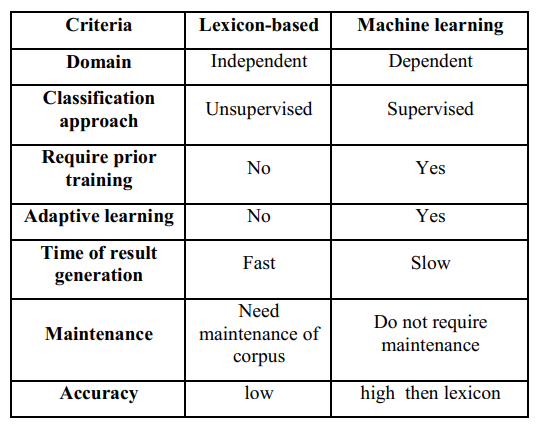
\includegraphics[width=0.5\linewidth]{images/lex_vs_ml.png}
  \caption{Comparison between lexicon and machine learning}
  \label{tab:sent_analysis_approaches}
\end{table}

Currently Sentiment analysis techniques seek to classify text as either positive, negative or neutral, using methods in Natural language processing (NLP). The common approach implemented involves statistical analysis and machine learning methods.\cite{ref2}

%
However people often express a particular emotion towards a certain topic. Specific emotions such as anger can lead to social unrest. This is undesirable but it can be helpful if we are able to quickly detect this before it occurs.
%
The proposed system will be a hybrid system it will use both machine learning approach as well as lexicon-based approach to detect both sentiment polarity and emotion.


\clearpage



\section{Lexicon (VaderSentiment)}
A lexicon is a collection of information about the words of a language about the lexical categories to which they belong. Lexicon based sentiment analysis makes use of labeled text this is very useful in detecting sentiment by emoticons. 
%
VaderSentiment is a python library that can be used to achieve this.\\ \\
VADER (Valence Aware Dictionary and sEntiment Reasoner) is a lexicon and rule-based sentiment analysis tool that is specifically attuned to sentiments expressed in social media.
VADER makes use of sentiment lexicon, which is a list of lexical features such as words, these words are labeled according to their sentiment polarity, positive, neutral or negative.
 \\ \\
An emoticon, short for "emotion icon", also known simply as an emote, is a pictorial representation of a facial expression using characters usually punctuation marks, numbers and letters to express a person's feelings or mood, or as a time-saving method rather than to type out a whole word, an emoticon can be used to convey the writer's feelings or intended tone. \\ \\

Some key features of Vader sentiment are: -

\begin{enumerate}

\item
Punctuation: The use of an exclamation mark(!), increases the magnitude of the intensity without modifying the semantic orientation. For example, “The food here is good!” is more intense than “The food here is good.” and an increase in the number of (!), increases the magnitude accordingly.

\item
Capitalization: Using upper case letters to emphasize a sentiment-relevant word in the presence of other non-capitalized words, increases the magnitude of the sentiment intensity. For example, “The food here is GREAT!” conveys more intensity than “The food here is great!”
\item
Degree modifiers: Also called intensifiers, they impact the sentiment intensity by either increasing or decreasing the intensity. For example, “The service here is extremely good” is more intense than “The service here is good”, whereas “The service here is marginally good” reduces the intensity.
\item
Conjunctions: Use of conjunctions like “but” signals a shift in sentiment polarity, with the sentiment of the text following the conjunction being dominant. “The food here is great, but the service is horrible” has mixed sentiment, with the latter half dictating the overall rating.
\item
Preceding Tri-gram: By examining the tri-gram preceding a sentiment-laden lexical feature, we catch nearly 90\% of cases where negation flips the polarity of the text. A negated sentence would be “The food here isn’t really all that great”.
\end{enumerate}

\clearpage
\subsection{Subjectivity and Objectivity (TextBlob)}
Subjectivity and objectivity differentiates opinionated and factual based text.\cite{ref2}
Being able to detect subjectivity and objectivity is an important part of sentiment analysis, because it can tell us more about the authors emotions and intentions, a subjective person is more likely to invoke action than an objective person. TextBlob python library can be used to detect the degree of subjectivity and the degree of objectivity, these results together with the polarity scores will be used to determine the impact of the sentiment. 

\clearpage
\subsection{Multi-label convolutional neural network text classifier (Spacy)}

SpaCy is a free, open-source library for advanced Natural Language Processing (NLP) in Python \\
Spacy makes use of a neural network text classifier. SpaCy can be used to categorize documents into the different emotion classes.
The Neural network is trained using stochastic gradient descent where the estimate of the error used to update the weights is calculated based on a subset of the training dataset. \\


\begin{figure}[h]
  \centering
  \pgfimage[width=0.7\linewidth]{images/sgd}
  \caption[Stochastic Gradient decent]%
  {Stochastic Gradient decent}
  \label{fig:ALAP:sm3}
\end{figure}






A SpaCy model uses statistical decisions to make predictions, the decision is based on examples used to train the model. Training the model requires training data, training data is: examples of text with the labels that we want to predict. This will be in the following categories
\begin{itemize}
\item "anger"
\item "disgust"
\item "fear"
\item "sadness"
\item "shame"
\item "joy"
\item "guilt"
\end{itemize}




The following diagram shows how SpaCy model is trained

\begin{figure}[h]
  \centering
  \pgfimage[width=0.7\linewidth]{images/spacy_training}
  \caption[SpaCy Training]%
  {SpaCy Training:https://spacy.io/usage/training}
  \label{fig:ALAP:sm3}
\end{figure}
 
\clearpage

\subsection{Training Dataset (ISEAR)}


Robert Plutchik invented a wheel of emotions. He suggested eight primary emotions: joy opposite to sadness. Similarly, anger opposite to fear; trust opposite to disgust and surprise opposite to anticipation. These four opposite emotion pairs, show the 8 basic emotions. Additionally, Plutchik’s model shows connections between the ideas of circle of emotions using a color wheel. Like the case of colors, primary emotions can also be expressed at different degrees of their intensities, for each emotion there are three degrees. For example, serenity is a less intense degree of joy
and ecstasy is a more intense degree of joy. Plutchik’s emotions can be mixed with one another
forming a new different emotion. For example, combination of joy and trust resulted to form a new
emotion ‘love’. Likewise, joy, anger and trust are combined and form jealousy\cite{ref:4}.

\begin{figure}[h]
  \centering
  \pgfimage[width=0.7\linewidth]{images/emotion_wheel}
  \caption[Robert Plutchik's wheel of emotions]%
  {Robert Plutchik's wheel of emotions}
  \label{fig:ALAP:sm3}
\end{figure}


ISEAR (International Survey on Emotion Antecedents and Reactions) is an open dataset collected by Klaus R. Scherer and Harald Wallbott. 
ISEAR dataset contains seven major emotions based on Robert Plutchik's wheel of emotions : joy, fear, anger, sadness, disgust, shame, and guilt.\\
It has over 7,600 entries for the emotion classes. This will be a good training dataset for emotion detection.
\clearpage

\subsection{Streaming twitter (tweepy)}
Tweepy is an open source python library that can be used to stream tweets from twitter in real time through the Twitter API.


\subsection{Confusion matrix}
A confusion matrix is used in machine learning to determine the performance of a classification algorithm. It is a tabular form than compares test data for which its true values are known. I will use the confusion matrix to evaluate the performance of my classification model.

A confusion matrix consists of the following classes.
 \begin{itemize}

\item
true positives (TP): This is when we have given a correct positive prediction

\item
true negatives (TN): This is when we have given a correct negative prediction.

\item
false positives (FP): This is when we have predicted yes, but the true value is no

\item
false negatives (FN): This is when we have predicted no, but the true value is yes

\end{itemize}

\begin{figure}[h]
    \centering
    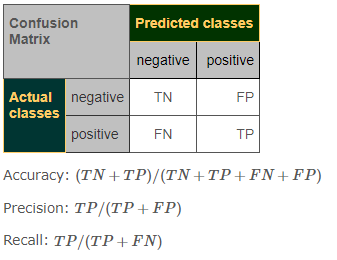
\includegraphics{images/confusion_matrix.png}
    \caption{Confusion matrix}
\end{figure}

  The above table shows how to determine the accuracy of the prediction using a confusion matrix. However, there are problems with accuracy. It assumes equal costs for both kinds of errors that is to say it assumes that we have an equal number of positives and negatives. A 99\% accuracy can either be excellent, good, mediocre, poor or terrible depending upon the problem
\clearpage
In the case of having multiple classes the confusion matrix becomes


\begin{figure}[h]
    \centering
    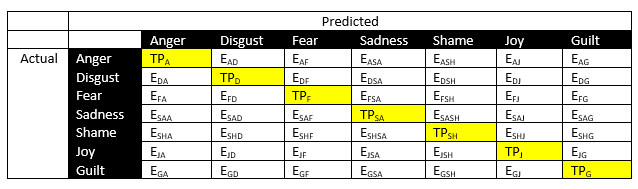
\includegraphics{images/confusion_matrix_2.png}
    \caption{Confusion matrix with multiple classes}
\end{figure}

Things to notice about a confusion matrix with multiple classes
\begin{itemize}
\item \textbf{total number of test examples} of any class if given by the sum of the corresponding row \textbf{(i.e TP + FN)}
\item \textbf{Total number of False Negatives} for a class is the sum of values in the corresponding row excluding the \textbf{True positives}

\item \textbf{Total number of false positives} for a class is the sum of values in the corresponding column excluding the \textbf{true positives}

\item \textbf{Total number of true negatives} for a certain class will be the sum of all columns and rows  excluding that classes column and row
\end{itemize}
  
\textbf{Accuracy} calculated as the sum of correct classifications divided by the total number of classifications\\
\textbf{Precision} is calculated as \textbf{ TP/(TP+ FP)}\\
\textbf{Recall} also called sensitivity, corresponds to the tue positive rate of the considered class
\\
calculated as Recall=Sensitivity=TP/(TP+FN)

\clearpage



\chapter{Sentiment analysis}

\subsection{Implementing (VaderSentiment and TextBlob)}


Using \textbf{"VaderSentiment"} library. Using an analyzer object, and looping through the list of tweets  calling the analyser.polarity\_scores() method and appending the results to an array.

\begin{lstlisting}
from vaderSentiment.vaderSentiment import SentimentIntensityAnalyzer
analyser = SentimentIntensityAnalyzer()#create the vader sentiment analyser object
sentiment_vs_tweets=[]#array will hold the processd tweets with the sentiment and objective labels
index=0
for t in tweets:
    sentiment_vs_tweets.append( analyser.polarity_scores(t) )#add the processed tweet to the list
    print(sentiment_vs_tweets[index])#print the sentiment polarity and subjecivity
    index=index+1
\end{lstlisting}


The above code will produces the following results

\begin{lstlisting}
{'neg': 0.252, 'neu': 0.581, 'pos': 0.168, 'compound': -0.3182}
{'neg': 0.0, 'neu': 1.0, 'pos': 0.0, 'compound': 0.0}
{'neg': 0.194, 'neu': 0.806, 'pos': 0.0, 'compound': -0.5574}
{'neg': 0.0, 'neu': 1.0, 'pos': 0.0, 'compound': 0.0}
{'neg': 0.194, 'neu': 0.806, 'pos': 0.0, 'compound': -0.5574}
\end{lstlisting}




Using \textbf{TextBlob} to detect the degree of subjectivity and objectivity of the documents.


\begin{lstlisting}
#here we use TextBlob python library to detect sentence/tweet/document polarity as well as subjectivity and store the results
#textblob uses a machine learning approach
from textblob import TextBlob
sentiment_tb_tweets=[]#array will hold the processd tweets with the sentiment and objective labels
index=0
for t in tweets:
    sentiment_tb_tweets.append( TextBlob(t) )#add the processed tweet to the list
    print(sentiment_tb_tweets[index].sentiment)#print the sentiment polarity and subjecivity
    index=index+1
    
sentiment_tb_tweets[0].subjectivity
\end{lstlisting}


The above code produces the following results


\begin{lstlisting}[language=Python]
Sentiment(polarity=0.0, subjectivity=0.25)
Sentiment(polarity=0.14285714285714285, subjectivity=0.31785714285714284)
Sentiment(polarity=0.0, subjectivity=0.06666666666666667)
Sentiment(polarity=0.2, subjectivity=0.2)
Sentiment(polarity=0.0, subjectivity=0.06666666666666667)
\end{lstlisting}

\clearpage

\subsection{Training SpaCy Text classifier}
Using the ISEAR training data
We can train a SpaCy model to classify text into some categories
\begin{figure}[h]
  \centering
  \pgfimage[width=0.5\linewidth]{images/isear}
  \caption{Sample ISEAR training dataset with labels}
  \label{fig:ALAP:sm1}
\end{figure}

We begin training the SpaCy model on the above training set,
start by reading in the data 
\begin{lstlisting}
nlp    = spacy.load('en_core_web_sm')#load english model
file    = open("data/train_data.txt","r")#read in training set from text file uses pipe delimiter
#read in the training set with the labels
for row in f_data:
    train_data.append( (row.split('|')[0],\
                        {"cats":\
                         {\
                          "anger"    :int(row.split('|')[1]),\
                          "disgust"  :int(row.split('|')[2]),\
                          "fear"     :int(row.split('|')[3]),\
                          "sadness"  :int(row.split('|')[4]),\
                          "shame"    :int(row.split('|')[5]),\
                          "joy"      :int(row.split('|')[6]),\
                          "guilt"    :int(row.split('|')[7])\
                        }}) )
                        
\end{lstlisting}
\clearpage
We then update the nlp model with the new training set
\begin{lstlisting}
#create the spacy nlp pipeline
textcat = nlp.create_pipe('textcat')
#add the pipeline to the nlp model| last=true since we want to add these conponents at the end of the model
nlp.add_pipe(textcat, last=True)
#declare the lables/categories
textcat.add_label('anger')
textcat.add_label('disgust')
textcat.add_label('fear')
textcat.add_label('sadness')
textcat.add_label('shame')
textcat.add_label('joy')
textcat.add_label('guilt')

optimizer = nlp.begin_training()
#next we will update the model with our own train_data from the csv file
for itn in range(1):
    for doc, gold in train_data:
        random.shuffle(train_data)
        losses = {}
        index = 0
        for text, annotations in train_data:
            nlp.update([doc], [gold], sgd=optimizer, drop=0.45, losses=losses)#drop rate at .45
            print("Iteration: {0}, %{1:.2f} Complete".format((itn+1), index/len(train_data) * 100))#show the progress
            index += 1
        print(losses)
 
\end{lstlisting}


After training the model we can now run some tweets via the model 
\begin{lstlisting}
#determine the class of the tweets using the spacy model trained earlier
#create a document and run it thru the nlp pipeline 
classified_tweets = []#array will hold the spacy classified tweets
index=0
for t in tweets:
    classified_tweets.append(  nlp(t) )
    print( classified_tweets[index].cats )#print the categories/classes of the document
    index=index+1  
\end{lstlisting}

The above code produces the following results
\begin{lstlisting}
{'anger': 0.8638094067573547, 'disgust': 0.41107258200645447, 'fear': 0.007243141997605562, 'sadness': 0.04211084172129631, 'shame': 0.7023115158081055, 'joy': 0.6675902605056763, 'guilt': 0.9010916352272034}
{'anger': 0.7449342012405396, 'disgust': 0.4830150306224823, 'fear': 0.016353892162442207, 'sadness': 0.2870638370513916, 'shame': 0.40636202692985535, 'joy': 0.1324012577533722, 'guilt': 0.41464924812316895}
{'anger': 0.7480689883232117, 'disgust': 0.4755619764328003, 'fear': 0.035106029361486435, 'sadness': 0.1592441201210022, 'shame': 0.4828783869743347, 'joy': 0.16910341382026672, 'guilt': 0.4793942868709564}
{'anger': 0.7859129905700684, 'disgust': 0.47182315587997437, 'fear': 0.026509756222367287, 'sadness': 0.32458046078681946, 'shame': 0.12689484655857086, 'joy': 0.23759214580059052, 'guilt': 0.9908844828605652}
{'anger': 0.7480689883232117, 'disgust': 0.4755619764328003, 'fear': 0.035106029361486435, 'sadness': 0.1592441201210022, 'shame': 0.4828783869743347, 'joy': 0.16910341382026672, 'guilt': 0.4793942868709564}
\end{lstlisting}

SpaCy model is able to classify the class of the text based on our training set



\clearpage

\subsection{Streaming twitter API(Tweepy)}

The python library tweepy can support accessing Twitter via Basic Authentication and the newer method, OAuth. The API parameters allow filtering tweets based on language, geolocation and tweets containing a particular word or phrase.

\begin{lstlisting}
auth   = OAuthHandler(consumer_key, consumer_secret)
auth.set_access_token(access_token, access_token_secret)

stream = Stream(auth, listner)
#run this code async 
streamer=stream.filter(track=search_terms,is_async=True,languages=langs,locations=loca_tions)
\end{lstlisting}

The listener object is a class that inherits from StreamListener class, it listens for any incoming tweets, cleans the tweets and then stores them in an array.

\begin{lstlisting}
class StdOutListener(StreamListener):
    def on_data(self, data):
        obj = json.loads(str(data))#convert the tweet into a json format
        #clean the tweets before inserting into the array
        clean_tweet = remove_pattern(obj["text"],"@[\w]*")#remove twitter handles (@user)
        clean_tweet = clean_tweet.replace("[^a-zA-Z#]", " ")#replace puntuation marks
        clean_tweet = clean_tweet.replace("RT :","")#replace the re tweet symbol
        clean_tweet = re.sub('http[s]?://(?:[a-zA-Z]|[0-9]|[$-_@.&+]|[!*\(\),]|(?:%[0-9a-fA-F][0-9a-fA-F]))+', '', clean_tweet, flags=re.MULTILINE)#remove hyperlinks
        
        score       = vs_analyser.polarity_scores(clean_tweet)
        sentiment_polarity_scores.append( float(score["compound"]) )#append the sentiment score to the array
        sentiment_tb_tweets.append( TextBlob(clean_tweet) )#append the texblob object to the array
        sentiment_vs_tweets.append( nlp(clean_tweet) )#append the vader sentiment object to the array
        tweets.append(clean_tweet)#append the clean tweet to the list of tweets
\end{lstlisting}



%%%%%%%%%%%%%%%%%%%%%%%%%%%%%%%%%%%%%%%%%%%%%%%%%%%%%%%%%%%%%%%%%%%%%%%
\subsection{Evaluating SpaCy classification model}\label{sec:THEORY:linear}
Because of the huge size of the training dataset, using the whole data set to train and evaluate the model would take too long. The solution therefore is to use a small sample of the dataset to train and evaluate.
The training set has 23 samples and the evaluation set has 8 samples.\\
The following is the results of the evaluation based on the confusion matrix.

\begin{lstlisting}
Accuracy:  1.4285714285714286



Precision_anger:  0.6666666666666666
Precision_disgust:  1.0
Precision_fear:  0.4
Precision_sadness:  1.0
Precision_shame:  1.0
Precision_joy:  1.0
Precision_guilt:  1.0
Total_Precision:  0.8666666666666666



Recall_anger:  1.0
Recall_disgust:  0.6666666666666666
Recall_fear:  1.0
Recall_sadness:  0.5
Recall_shame:  0.5
Recall_joy:  0.5
Recall_guilt:  0.5
Total_Recall:  0.6666666666666666
\end{lstlisting}

The results for each individual classification is quite satisfactory, considering that the training set and evaluation set is considerably small. Both the precision and the Recall is 50\% and above.






%!TEX root = francis_thesis.tex
%%%%%%%%%%%%%%%%%%%%%%%%%%%%%%%%%%%%%%%%%%%%%%%%%%%%%%%%%%%%%%%%%%%%%%%
\chapter{Results and analysis}\label{ch:Results}


\section{Used Technologies}
Various technologies, frameworks and libraries were used in this project. Every implementation was carried out in Python, and frameworks like TensorFlow and Keras were used. Below are the list of the technologies used and a brief description.

\subsection{Python}

\begin{figure}[H]
    \centering
    
\includegraphics[width=0.8\linewidth]{images/python-logo.png}
     \caption{Python logo, source: https://www.python.org/community/logos/}
  \end{figure}

Python\footnote{https://www.python.org/community/logos/} is a high level programming language designed by Guido van Rossum in 1991. Its design philosophy emphasizes code readability and has a remarkable use of significant whitespace. The filename extensions include .py, .pyc, .pyw, .pyz. It support web development with frameworks like Django and Pyramid. It is applied in scientific studies and machine learning. Several libraries and frameworks have been developed by the Python community for this such as 
SciPy\footnote{www.scipy.org}, Scikit-learn\footnote{scikit-learn.org/stable/}, Pandas\footnote{pandas.pydata.org}, Numpy\footnote{www.numpy.org/}, Theano\footnote{deeplearning.net/software/theano/}, PyTorch \footnote{pytorch.org/}, etc. It is also one of the most popular languages in the field of Convolutional neural network. Neural Networks like ResNet, VGGNet, Faster R-CNN, AlexNet in Keras or Pytorch, etc. 

\subsection{ TensorFlow}
\begin{figure}[H]
    \centering
    
\includegraphics[width=0.7\linewidth]{images/TensorFlow.png}
     \caption{TensorFlow logo, source: www.tensorflow.org}
  \end{figure}
TensorFlow\footnote{www.tensorflow.org} is an Apache Licensed library. It is free and open-sourced and developed by Google Brain Team. It is written in Python, C++ and CUDA. It is a symbolic math library applied for machine learning application such as deep neural network, convolutional neural network. TensorFlow was used in the implementation of the deep learning network for this project. TensorFlow has a comprehensive, flexible ecosystem of tools, libraries that makes it user-friendly.
For a wider documentation, please see the official website\footnote{www.tensorflow.org}
\clearpage

\subsection{Keras}
\begin{figure}[H]
    \centering
    
\includegraphics[width=0.9\linewidth]{images/keras.png}
     \caption{Keras logo, source:www.scikit-image.org}
  \end{figure}

Keras \footnote{Keras.io} is an MIT licensed neural-network library written in Python. It was design by Francois Chollet and released first in March 2015. It is open-sourced. Keras is capable of running on top of Microsoft Cognitive Toolkit, TensorFlow, PlaidML or Theano for fast experimentation of deep neural networks. It enables implementation of deep learning and allows easy and 
fast prototyping, supports both convolutional networks and recurrent networks and the combination of both. For a wider documentation, please see the official website\footnote{www.keras.io}

\subsection{ Scikit-Image}
\begin{figure}[H]
    \centering
    
\includegraphics[width=0.7\linewidth]{images/Scikit-image.png}
     \caption{Scikit-Image logo, source: www.scikit-image.org}
  \end{figure}

Scikit-Image is a BSD licensed image processing library. It is a collection of algorithms for segmentation, 
geometric transformations, analysis, filtering, colour space manipulation, morphology, feature detection, and so on. It was first released in 2009, written by Stefan van der Walt.
\cleardoublepage
\section{Implementation}
\subsection{Dataset}
Drones, or general UAVs, equipped with cameras have been fast applied to a wide range of applications, including agricultural, aerial photography, fast delivery, and surveillance. Consequently, automatic understanding of visual data collected from these platforms become highly demanding, which brings computer vision to drones more and more closely. 
Various computer vision task has been carried out by the Vision meets Drone (VisDrone) Challenges\footnote{www.aiskyeye.com}
organized  by the AISKEYE team at Lab of Machine Learning and Data Mining , Tianjin University, China in the year 2018.
Various computer vision task carried out in the challenge include object detection in images. The task aims to detect objects of predefined categories (e.g., cars and pedestrians) from individual images taken from drones. Also, object detection in videos challenge. The task is similar to the first, except that objects are required to be detected from videos. Then single-object tracking challenge. The task aims to estimate the state of a target, indicated in the first frame, in the subsequent video frames. And finally, multi-object tracking challenge. The task aims to recover the trajectories of objects in each video frame.
Originally, I wanted to use the dataset provided by VisDrone Challenge for the training and validation of my Mask R-CNN Network, but due to lack of the segmentation mask data for the training set, I couldn’t use it.
Rather I made use of the Semantic Drone Dataset from Institute of Computer Graphics and Vision, Graz University of Technology, Austria. \footnote{dronedataset.icg.tugraz.at}

\paragraph{}
The dataset contains images, bounding boxes as python pickle file, bounding boxes as xml, bounding boxes as mask images. The Semantic Drone Dataset focuses on semantic understanding of urban scenes for increasing the safety of autonomous drone flight and landing procedures. The imagery depicts  more than 20 houses from nadir (bird's eye) view acquired at an altitude of 5 to 30 meters above ground. A high resolution camera was used to acquire images at a size of 6000x4000px (24Mpx). The training set contains 400 publicly available images and the test set is made up of 200 private images. [W]
For the task of person detection the dataset contains bounding box annotations of the training and test set. And for semantic segmentation, pixel-accurate annotation for the same training and test set was prepared. The complexity of the dataset is limited to 20 classes as listed below.

\begin{itemize}
  \item tree
  \item tree
  \item grass
  \item other vegetation
  \item dirt
  \item gravel
  \item rocks
  \item water
  \item paved area
  \item pool
  \item person
  \item dog
  \item car
  \item bicycle
  \item roof
  \item wall
  \item fence
  \item fence-pole
  \item window
  \item door
  \item obstacle
  
\end{itemize}
The Drone Dataset is made freely available to academic and non-academic entities for non-commercial purposes such as academic research, teaching, scientific publications, or personal experimentation.
\paragraph{}
For the implementation of the instance segmentation, Python was used for obvious reasons. It enabled me to use deep learning framework like Tensorflow and Keras. The implementation of the model was carried out in the file drone.py and uses the Mask R-CNN library developed in python with TensorFlow and Keras by Matterport Inc. It was written by Waleed Abdulla from Matterport Inc. Matterport, Inc. published their implementation under the MIT License [X]. The MIT License is a license granting the permission to use the code, copy it, modify it, publish and even to sell it free of charge.
There's absolutely no restriction on commercial use in MIT license. The only requirement is that you must include the MIT copyright notice with any copies of the software. Scripts, files and noteboks in the library are also under the MIT License and moreover, Waleed Abdulla himself agreed with the usage and modifications of his code for purposes of the research work.The Matterport, Inc. Mask R-CNN implementation can be found in their GitHub repository.
Moreover, the Matterport implementation of Mask R-CNN was selected because of several reasons. Besides its license compatibility, it is quite robust and ready for modifications and adaptation for training in drone dataset leading to another implementation, so it saved thousands of lines of code. One of the major motivation behind its usage is that there is a plenty of people interested in this project, proposing their ideas and testing it. And these people are experienced in fields of computer vision and deep learning. Abdulla himself is responsive and active in answering people’s questions and issues. He is open-minded when discussing other people improvement proposals. I found it very useful.
The next section will discuss the Mask R-CNN library, the workflow and necessary module of the library. The structure, architecture and components of the Mask R-CNN have been discussed in Chapter 2, so explanation of the programs only will be given in the next section. The library will be also discussed altogether with notes on my modifications connected with this thesis to distinguish them from Abdulla’s code.

\subsection{Mask R-CNN library}
The library which is hosted in Github has been forked 5445 times. It contains five important modules. Each module play an important role in the training and testing of model. Let’s go through this modules on after the other below:
\\
\textbf{Config.py}
\\
This is the configuration module of the system. It includes hyper-parameters for tuning of the model and necessary setting. It will described in section 4.2.1SS
\\
\textbf{Model.py}\
This is fundamental core of the model. It develops and builds up the model. It will described in section 4.2.2
\\	
\textbf{Parallel\_Model.py}\ 
This module subclasses the standard Keras Model and adds multi-GPU support. It works by creating a copy of the model on each GPU and creates a parallelized computation.
This file was not modify further and so will not explained in this thesis.
\\
\textbf{Utils.py} \
This modules contains the utility classes and functions of the model. It will described in section 4.2.3
\\
\textbf{Visualize.py}\
This contains function for display and visualization. It will described in section 4.2.4
\\

The python files for the modules have good inner documentation, of which some of them and other functionalities will be discussed next.

\subsubsection{Config.py}
Config.py is the configuration settings for the model in the implementation by Matterport Inc.. It contains the hyper-parameters of the model. It has a classed called ModelConfig that houses these parameters. These parameter include;
 \begin{itemize}
   \item GPU Count
   \item Images per GPU
   \item Steps per Epoch
   \item Validation steps
   \item The choice of the backbone
   \item Backbone strides (The strides of each layer of the Feature Pyramid Network (FPN) pyramid discussed in section 2.2)
   \item Learning Rate
   \item RPN Train Anchors Per\_ Image (How many anchors per image to use for RPN training)
   \item Mask Shape
   \item And so on.
   
 \end{itemize}
 I inherited ModelConfig  class and then adapted the attributes to suit my hardware and the drone-based dataset in the drone.py module.  The config.py also a contains a display function that displays the model’s attribute.

 \subsubsection{Model.py}
 This is the main Mask R-CNN implementation. It is made use of some modules for its implementation which include, os, random, datetime, re, logging, collections, multiprocessing ,numpy,tensorflow, keras, keras.backend ,keras.layers ,keras.engine , ,keras.models. distutils.version. For the module to work it needs TensorFlow 1.3+ and Keras 2.0.8+ .  Since this module builds the Mask R-CNN it has several classes and function performing various tasks. This classes and task the perform can be summed up thus;
 \begin{itemize}
   \item 	Initialization functions
   \item Building the ResNet backbone.
   \item Building the RPN.
   \item Building RoIAlign layers.
   \item Building head architectures.
   \item Building the complete Mask R-CNN model and putting everything together.
   \item Building detection layers.
   \item Defining loss functions.
   \item	Data formatting
   \item Miscellaneous functions and utilities connected to the model, like batch normalization data formatting and generating (building up targets, loading ground truth masks) or bounding boxes normalization.
   
 \end{itemize}
 Some important functions in the modules include train, load\_weight, build, etc. There was no modification made in this module for the training of model, apart from few modification to fix error that could be raised during the loading of masks. An explanation is given to the program written by Waleed Abdulla
\\ 
\\
\textbf{ RESNET}
\\
 The backbone of the Mask R-CNN is the Residual Network (RESNET). For the building of the RESNET, the principal function that does this is the resnet\_graph . The  resnet\_graph builds the ResNet graph and the  architecture can be ResNet50 or ResNet101.The batch norm layers of the network can be freeze or trained by setting the train\_bn to True or False, but the default is True. The workflow is outlined in pseudocode 4.1
 \\
\\

 \begin{algorithm}[H]
  \caption{Building the ResNet backbone architecture}
  \SetAlgoLined
  \DontPrintSemicolon
 layers = intended layers\;
 layers .add( zero padding 3x3)\;
 layers .add( convolution 7x7)\;   
 layers .add( batch normalization )\;
 layers .add( ReLu )\;
 layers .add( maximum pooling )\;
 layers .add( convolutional block 64 x64x256 )\;
 layers .add (2 identity blocks 64 x64x256 )\;
 layers .add( convolutional block 128 x128x512 )\;
 layers .add (3 identity blocks 128 x128x512 )\;
 layers .add( convolutional block 256 x256x1024 )\;
\uIf{architecture == ’resnet50 ’}{
  layers .add (5 identity blocks 256 x256x1024 )\;
}
\uElseIf{architecture == ’resnet101 ’}{
  layers .add (22 identity blocks 256 x256x1024 )\;
}


return layers\;   
 \end{algorithm}
.\\
\\
The genuine function does not return total layers, however, it returns them in stages  C1, C2, C3, C4, C5 as can be seen in pseudocode 4.8, where this function is called  build\_resnet\_backbone. Every one of these stages speaks to the condition of craftsmanship before each convolutional block expansion, which is the last layer before changing components of input or yields. It is significant for the FPN as was referenced in Chapter 2 what's more, outlined in the model structure in pseudocode 4.8. Functions identity block and convolutional block are fundamentally the same as and both fabricates the bottleneck block. The main contrast is that the convolutional block function likewise actualizes a 1x1 convolution in the alternate route association as it is important to change the state of the contribution to the one utilized in the block. The remainder of their usage is pretty much the equivalent and is represented in pseudocode .2 (the convolution ought to be connected in the yield association step). It uses channels given to each call of the capacity in the ResNet pseudocode.
\\
\\
\begin{algorithm}[H]
  \caption{identity\_block}
  \SetAlgoLined
  \DontPrintSemicolon
  original\_input = original\_input\_tensor\;
  block = intended block of layers\;
   block .add ( convolution 1x1)\;
   block .add ( batch normalization )\;
   block .add ( ReLu )\;
   block .add ( convolution 3x3)\;
   block .add ( batch normalization )\;
   block .add ( ReLu )\;
   block .add ( convolution 1x1)\;
    block .add ( batch normalization )\;
   block . connect\_outputs (block , original\_input )\;
   block .add ( ReLu )\;
   return block\;
  
  \end{algorithm}
.\\
\\
 \textbf{RPN}
\\
The RPN is worked by two functions, build\_rpn\_model and rpn\_graph. Notwithstanding, these functions assemble just the model, for example, the sliding window and its behavior, anchors are created in utils.py as depicted in section 5.1.3. Indeed, even in this split approach, it pursues the thought from section 3.4.3. Contributions for the rpn\_graph capacity are an element map, number of anchors per area and anchors stride and returns anchors class logits, probabilities and bounding boxes refinements. The work process of rpn\_graph is represented in pseudocode 5.3. build\_rpn\_model makes a model which initially feed the rpn\_graph work and at that point restores the previously mentioned qualities.
\\
\\
\begin{algorithm}[H]
  \caption{rpn\_graph}
  \SetAlgoLined
  \DontPrintSemicolon
  feature\_map = input\_feature\_map\;
  logits\_number\_of\_filters = 2 * number of anchors per location\;
   bbox\_number\_of\_filters = 4 * number of anchors per location\;
   shared\_layer = convolution 3x3 on feature\_map\;
   rpn\_class\_logits = convolution 1x1 on shared\_layer with logits\_number\_of\_filters\;
  rpn\_probabilities = softmax on rpn\_class\_logits\;
   rpn\_bbox\_refinements = convolution 1x1 on shared\_layer with bbox\_number\_of\_filters\;
   return rpn\_class\_logits , rpn\_probabilities , rpn\_bbox\_refinements\;
  
  \end{algorithm}
  .\\
\\
  A significant class for the RPN is the ProposalLayer class. It takes anchor probabilities, bounding box refinements and anchors themselves as inputs trim them to littler clumps while considering top anchors and applies refinements to the anchor boxes.
\\
\\
\begin{algorithm}[H]
  \caption{ProposalLayer}
  \SetAlgoLined
  \DontPrintSemicolon

probs = anchor probabilities\;
deltas = anchor refinements\;
anchors = anchors\;
threshold = threshold for probabilities\;
top\_anchors = names\_of\_anchors\_with\_top\_probs (probs , how\_many =min(6000 , len( probs )))\;
 probs\_batch = batch\_slice (probs , top\_anchors )\;
 deltas\_batch = batch\_slice (deltas , top\_anchors )\;
 anchors\_batch = batch\_slice ( anchors , top\_anchors )\;
 boxes = apply\_refinements ( anchors\_batch , deltas\_batch )\;
 proposals = [boxes , probs\_batch ]\;
 proposals . apply\_threshold ( threshold )\;
 return proposals\;

  \end{algorithm}
  .\\
  \\
\clearpage
 \textbf{ROIAlign}
\\
As was described already in chapter 2, RoIAlign is more or less the RoIPooling algorithm without rounding. The implementation is briefly sketched below
\\
\\
\begin{algorithm}[H]
  \caption{RoIAlign}
  \SetAlgoLined
  \DontPrintSemicolon
pool\_shape = shape of regions\;
 image\_shape = shape of the image\;
 boxes = list of RoIs\;
 feature\_maps = list of feature maps\;
 h, w = compute\_heights\_and\_widths\_boxes ( boxes )\;
 image\_area = image\_shape [0] * image\_shape [1]\;
 roi\_level = minimum (5, 4 + log2 ( sqrt (h * w) / (224 / sqrt (image\_area ))))\;
pooled = list ()\;
\For{\texttt{level in range (2, 6)}}{
 roi\_level\_i = 1 where roi\_level == level , 0 elsewhere\;
 level\_boxes = gather (boxes , indices = roi\_level\_i )\;
 pooled . append ( crop\_and\_resize ( original\_image = feature\_maps [level-2] , what\_process = level\_boxes , shape = pool\_shape , method =’
bilinear ’))\;}

pooled . rearrange\_to\_match\_the\_order ( boxes )\;
\textbf{return} pooled\;
\end{algorithm}
.\\
\\
It executes the RoIAlign algorithm on different dimensions of the feature pyramid furthermore, in its specifications of the \newcommand*{\logten}{\mathop{\log_{2}}} condition, it pursues the thoughts behind identifications in [27] and furthermore applies the five-levels approach. The base picking at line 7 and the loop at line 9 the then pursues utilizing just layers two to five from chapter 5.1.2.
\\
\\
\textbf{Head architectures}
\\
As can be found in figure 3.13 and was at that point portrayed in section 3.6.1, the head architecture is separated into two areas. The head architecture for bounding boxes what's more, class probabilities are dealt with by the fpn\_classifier\_graph function and the mask architecture by the build\_fpn\_mask\_graph. 
fpn\_classifier\_graph takes as input RoIs, feature maps, pool size and a number of classes and returns classifier logits, probabilities and bounding boxes refinements. build\_fpn\_mask\_graph takes a similar input yet returns just a rundown of masks.
\\
\\
\begin{algorithm}[H]
  \caption{fpn\_classifier\_graph}
  \SetAlgoLined
  \DontPrintSemicolon
  rois = given regions of interest in normalized coordinates\;
  feature\_maps = list of feature maps from layers P2 , P3 , P4 , P5\;
   pool\_size = height of feature maps to be generated from ROIpooling\;
  num\_classes = number of classes\;
  layers = list of keras layers\;
  layers .add( ROIAlign ( pool\_size , input =[ rois , feature\_maps ]))\;
   layers .add( convolution pool\_size X pool\_size )\;
   layers .add( batch\_normalization )\;
   layers .add( ReLU )\;
   layers .add( convolution 1x1)\;
   layers .add( batch\_normalizataion )\;
   layers .add( ReLU )\;
   shared = squeeze\_to\_one\_tensor ( output of layers )\;
   class\_logits = fully\_connected\_layer ( input =shared ,number\_of\_filters = num\_classes )\;
   probabilities = softmax ( class\_logits )\;
   bboxes = fully\_connected\_layer ( input =shared , number\_of\_filters =4 * num\_classes )\;
   return class\_logits , probabilities , bboxes\;
  
  
\end{algorithm}
.\\
\\
\begin{algorithm}[H]
  \caption{build\_fpn\_mask\_graph}
  \SetAlgoLined
  \DontPrintSemicolon
   rois = given regions of interest in normalized coordinates\;
   feature\_maps = list of feature maps from layers P2 , P3 , P4 , P5\;
   pool\_size = height of feature maps to be generated from ROIpooling\;
   num\_classes = number of classes\;
   layers = list of keras layers\;
   layers .add( ROIAlign ( pool\_size , input =[ rois , feature\_maps ]))\;
   layers .add( convolution 3x3)\;
   layers .add( batch\_normalization )\;
   layers .add( ReLU )\;
   layers .add( convolution 3x3)\;
   layers .add( batch\_normalization )\;
   layers .add( ReLU )\;
   layers .add( convolution 3x3)\;
   layers .add( batch\_normalization )\;
   layers .add( ReLU )\;
   layers .add( convolution 3x3)\;
   layers .add( batch\_normalization )\;
   layers .add( ReLU )\;
   layers .add( deconvolution 2x2 with strides 2)\;
   layers .add( convolution 1x1 with sigmoid as an activation function )\;
  
   \textbf{return} layers
\end{algorithm}
.\\
\\

In the pseudocodes above, a ROIAlign object is added as the first one into layers. This object was sketched in pseudocode 5.5.
\\
\\
\textbf{Mask R-CNN model}
\\
The focal point of the model.py record is the MaskRCNN class which contains techniques to manufacture the whole Mask R-CNN model by cobbling together various kinds of layers 
what's more, to utilize it for training or detection. The work process of the technique build is represented in pseudocode 5.8 and pursues 
the architecture portrayed in chapter 3.6.1. In the pseudocode, we can see that the head architecture contrasts a bit in the training and in the detection. It is expected to 
the way that we need loss values to be processed during the training, so we figure them from detected values and target values (values dependent on known focuses from 
the training dataset).
\\
\\
\begin{algorithm}[H]
  \caption{Mask R-CNN.build}
  \SetAlgoLined
  \DontPrintSemicolon
 C2 , C3 , C4 , C5 = build\_resnet\_backbone ()\;
 P5 , P4 , P3 , P2 = build\_top\_down\_fpn\_layers (C2 , C3 , C4 , C5)\;
 anchors = generate\_anchors ()\;
 rpn = build\_rpn ()\;
 rois = ProposalLayer (rpn , anchors )\;
 \eIf{ mode == 'training '}{
    ground\_truth\_values = values from the training dataset\;
    bbox , classes = fpn\_classifier ( rois )\;
    target\_detection = DetectionTargetLayer ( ground\_truth\_values )\;
  mask = fpn\_mask ( rois from target\_detection )\;
   loss = loss\_functions ( target\_detection , bbox , classes , mask )\;
   model = [bbox , classes , mask , loss ]\;
}{
     bbox , classes = fpn\_classifier ( rois )\;
     target\_detection = DetectionLayer (bbox , classes )\;
     mask = fpn\_mask ( rois )\;
    model = [bbox , classes , mask ]\;
 }
 \textbf{return} model\;
\end{algorithm}
.\\
\\ 
In the pseudocode, we can see a few classes and functions. Despite the fact that their motivations are very clear, some of them can be seen in various pseudocodes. Function
build\_resnet\_backbone was at that point depicted in pseudocode 5.1, ensuing function build\_top\_down\_fpn\_layers is genuinely clear procedure connecting layers 
as in section 3.6.1, generate\_anchors will be portrayed in 5.12, build\_rpn can be seen in pseudocode 5.3, ProposalLayer in pseudocode 5.4, fpn\_classifier speaks to the fpn\_classifier\_graph from pseudocode 5.6 and fpn\_mask is work 
build\_fpn\_mask\_graph from pseudocode 5.7.


%!TEX root = francis_thesis.tex
%%%%%%%%%%%%%%%%%%%%%%%%%%%%%%%%%%%%%%%%%%%%%%%%%%%%%%%%%%%%%%%%%%%%%%%
\chapter{Conclusion}\label{ch:PRACTICE}

\begin{summary}
The aim of this project is to automatically detect and segment objects in a drone-based dataset by extending the application of Mask R-CNN the drone-based dataset. With the advance of the applicability of drone to daily-life activities, industries and farms. Counting objects with drones is a new application of drone. This work aim to provide a system for object detection in drone-based dataset that can be practically applied in facilitating work performed by industries like agricultural, oil and gas industries and so on.  As a future work the model will be deployed in the drone developed by the Robotic Team of African University of Science and Technology (AUST) for detection and control of pipeline vandalism in oil and gas industries. 
The first part of the thesis was dedicated to a theoretical background behind
CNNs.It also discussed by the general overview of various computer vision tasks. The second part is dedicated to the introduction of tools used in the work and the implementation of Mask R-CNN modules using the technologies on drone-based datasets. More importantly explanation to most important parts of the code.
Developed modules are available in GitHub repository.  


\end{summary}


%%%%%%%%%%%%%%%%%%%%%%%%%%%%%%%%%%%%%%%%%%%%%%%%%%%%%%%%%%%%%%%%%%%%%%%




\appendix
%!TEX root = kudzai_thesis.tex



{ 
	\renewcommand{\baselinestretch}{0.8}\normalsize %
	\setlength{\itemsep}{-2.4mm}
	\setlength{\bibspacing}{0.67\baselineskip}
	\bibliographystyle{abbrvnat}
	\setcitestyle{numbers}
	\bibliography{thesis}
}

\end{document}
